\documentclass{article}

\usepackage{listings}
\usepackage{color}
\usepackage{graphicx}
\usepackage{float}
\usepackage{hyperref}
\graphicspath{ {images/} }

\definecolor{backcolor}{rgb}{0.95, 0.95, 0.95}

\lstdefinestyle{codestyle} {
    backgroundcolor=\color{backcolor}
}

\lstset{style=codestyle}

\title{
    Testing Policy\\
    \begin{large}
        \textit{Golf Course Mapper}
    \end{large}
}
\date{
    \begin{small}
        \today
    \end{small}
}
\author{
    Team Recursive Recursion
}

\begin{document}
    \pagenumbering{gobble}
    \maketitle
    \newpage
    \pagenumbering{arabic}
    
    \tableofcontents
    \newpage

    %===========================================================================

    \section{Introduction}
    \label{sec:intro}

    \subsection{Purpose}
    \label{sec:purp}

    This \textit{Testing Policy Document} is intended to be a guide on the
    testing procedure, tools and practices that are followed when working on
    the \textit{Golf Course Mapper} project. The remainder of this section
    describes the different repositories used within the project and the
    deployment pipeline used. The remainder of this document then continues to
    describe the testing policies applied to each individual repository,
    excluding the documentation repository.

    \subsection{Repositories Structure}
    \label{sec:reps}

    There are five (5) repositories that are used for the project:
    \texttt{web-app}, \texttt{mobile-app}, \texttt{ios-app},
    \texttt{mapper-api} and \texttt{documentation}. A short description of the
    contents of each repository is listed below.

    \begin{itemize}
        \item \texttt{web-app}
            \subitem Contains web application subsystem used for mapping and
            managing golf courses. The web application is built using
            \textit{Angular 6}.
        \item \texttt{mobile-app}
            \subitem Contains the \textit{Android} app used for viewing golf
            courses. The mobile app is built using native Java code.
        \item \texttt{ios-app}
            \subitem Contains the \textit{iOS} app used for viewing golf
            courses. The iOS app is built using native Swift code.
        \item \texttt{mapper-api}
            \subitem Contains the \textit{Entity Framework Core} API used to
            manage and provide access to the database. The database used is
            \textit{PostGIS}, an extention of \textit{PostgreSQL}.
        \item \texttt{documentation}
            \subitem Contains all documentation relating to the project,
            including this file. Documents are written in \LaTeX. The repository
            also contains all additional images and published PDF versions of
            the documents.
    \end{itemize}

    \subsection{Deployment Pipeline}
    \label{sec:pipe}

    A continuous deployment pipeline is set up using \textit{Azure DevOps}
    [1]. When code is pushed to the \texttt{master} branch of the
    \texttt{web-app} or \texttt{mapper-api} repositories, the deployment
    pipeline is triggered. Once triggered, the unit and integration tests are
    run for the repository. If the tests pass, the subsystem is built. If the
    build is successful, the build artifact is stored (used for reverting to
    previous builds if necessary) and a \textit{Docker} image is created. The
    server then pulls the new Docker image and performs any necessary
    maintenance before deploying the new release.

    Figure \ref{fig:deployment} shows the release management page of Microsoft
    Azure DevOps, where the history of builds for both the Web App and API can
    be viewed.

    \begin{figure}[H]
        \centering
        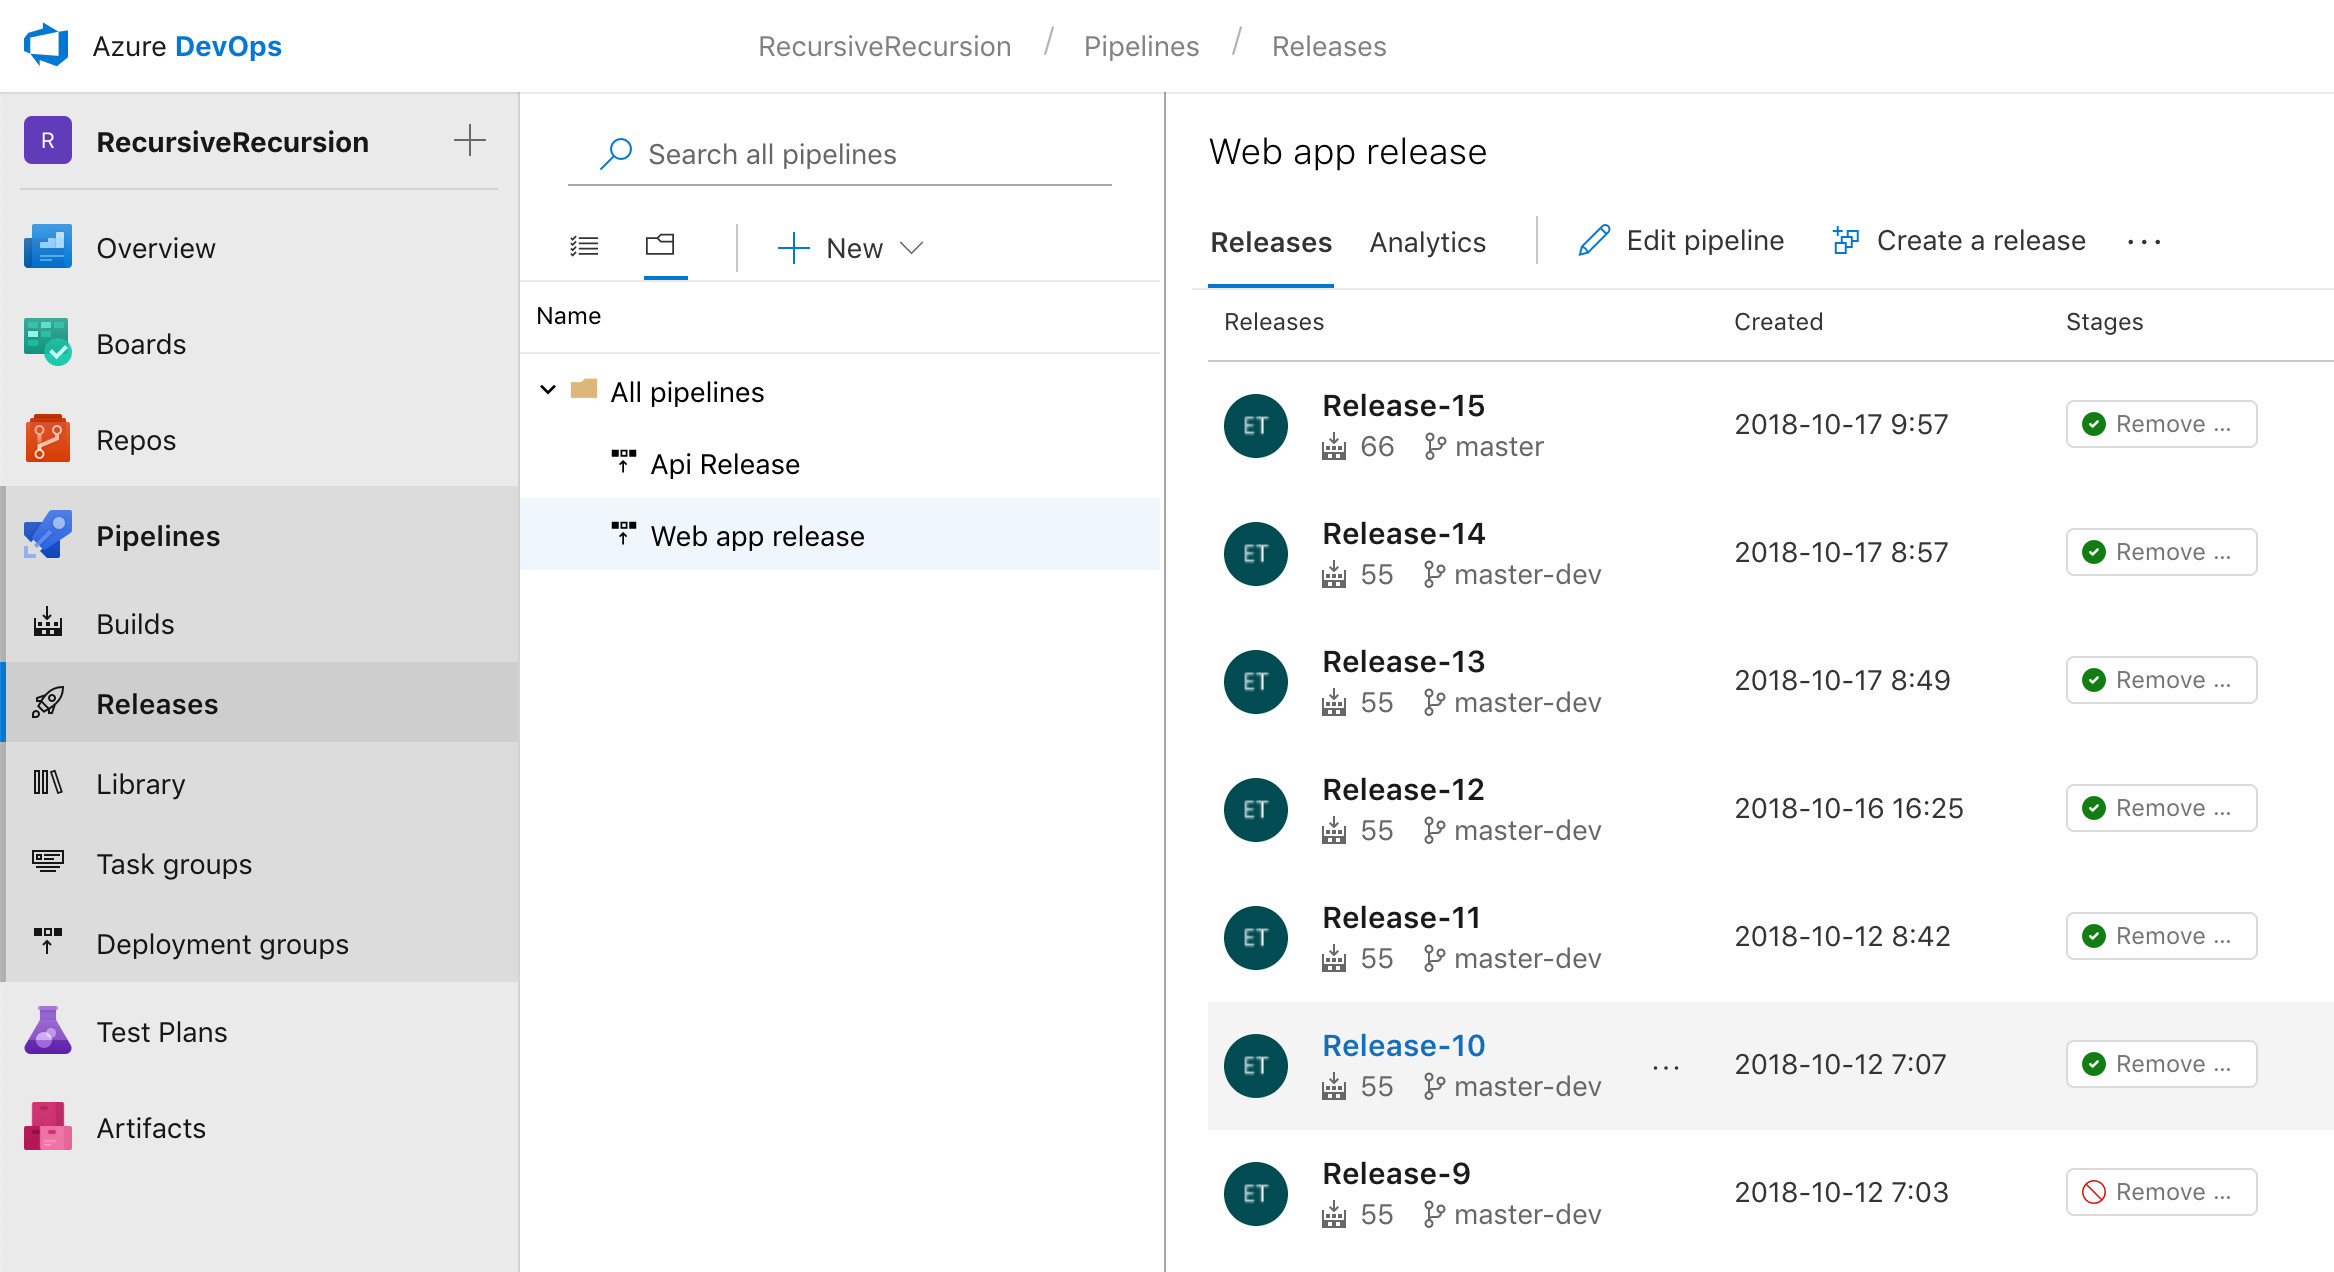
\includegraphics[scale=0.3]{Deployment}
        \caption{Continuous deployment}
        \label{fig:deployment}
    \end{figure}
    \newpage

    %===========================================================================

    \section{Testing Process}
    \label{sec:process}

    The following describes the process that is followed when testing code. The
    process described is the same for all repositories.

    \subsection{Targets}
    \label{sec:targets}

    The following tests are performed to ensure that the system is operating
    correctly and satisfies the functional requirements, as outlined in the
    \textit{Software Requirements Specification} (SRS) [2].

    \begin{itemize}
        \item \textit{Unit Tests} are performed to ensure that individual
            functions and components of each system component performs
            correctly.
        \item \textit{Integration Tests} are performed to ensure that the
            different subsystems operate correctly. This is further described
            in Section \ref{sec:mapper-api}.
        \item \textit{Acceptance Tests} are performed along with the client to
            ensure that the system meets the client's requirements and
            expectations.
    \end{itemize}

    The following tests are performed to ensure that the system complies with
    the non-functional system requirements, as outlined in the SRS.

    \begin{itemize}
        \item \textit{Usability Testing} is performed to receive feedback on
            the UI design of the web and mobile applications. This also ensures
            that the UI is as user-friendly as possible.
    \end{itemize}

    \subsection{Procedure}
    \label{sec:procedure}

    \paragraph{Unit tests} must be written and passed before code can be merged
    to the \texttt{master-dev} branch. This ensures that code on the dev branch
    is at least functionally correct. For details on how unit tests are
    performed for the Android app and Zoning API, see the sections
    \ref{sec:mobile-app} and \ref{sec:mapper-api}, respectively.

    \paragraph{Integration tests} must be passed before code can be pushed to
    the the \texttt{master} branch for deployment. This ensures that code on
    the master branch is always in a usable state. For details on how
    integration tests are performed, see Section \ref{sec:mapper-api}.

    \paragraph{Acceptance tests} are performed monthly with the clients to
    verify that the system complies with their requirements.

    \paragraph{Usability testing} is performed at least once close to the
    initial release of the system. For details on the usability test performed,
    see section \ref{sec:wa-tools}.

    \newpage

    %===========================================================================

    \section{Web App Testing}
    \label{sec:web-app}

    This section describes the testing policies adopted in the \texttt{web-app}
    repository. Being a subsystem that mainly acts as a frontend, only
    usability tests are performed. The history of the tests are shown in
    Section \ref{sec:wa-hist}.

    \subsection{Usability Testing}
    \label{sec:wa-tools}

    In order to satisfy the usability requirement of the system, it is
    necessary to perform a usability test to ensure that the system is
    user-friendly enough to non-technical users. A formal usability test is
    performed, asking testers to perform specific tasks on the system.
    
    Testers are then asked to provide critical feedback on the system, which is
    then analyzed. The results are then used to identify key issues in the
    design of the user interface.

    \subsection{History}
    \label{sec:wa-hist}

    Figure \ref{fig:usability} illustrates the usability test performed on 20
    September, 2018. Six testers from various backgrounds were asked to perform
    a serious of tasks on the web application, without any prior introduction
    to the user interface. The testers were then given a form to fill out,
    asking them to provide any feedback. The results of the test have been compiled
    in the Usability Report [3].

    \begin{figure}[H]
        \centering
        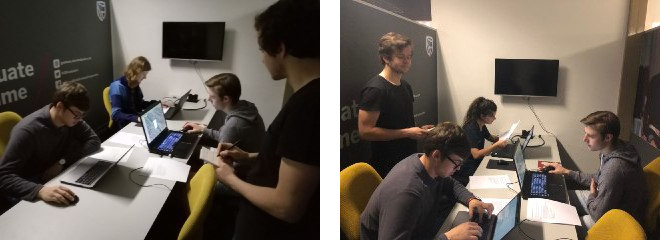
\includegraphics[scale=0.55]{UsabilityTest}
        \caption{Usability test in progress}
        \label{fig:usability}
    \end{figure}

    \newpage
    
    %===========================================================================

    \section{Mobile App Testing}
    \label{sec:mobile-app}

    This section describes the testing policies adopted in the
    \texttt{mobile-app} repository. The tools used for testing are described in
    Section \ref{sec:ma-tools}.  The layout of the test cases and history of
    the tests are shown respectively in Sections \ref{sec:ma-cases} and
    \ref{sec:ma-hist}.

    \subsection{Tools}
    \label{sec:ma-tools}

    The mobile app uses \textit{JUnit} to perform unit tests on the Android
    app. The built-in unit test functionality of \textit{Android Studio} is
    used to automate the testing process. The tests are run by selecting
    UnitTests in the build options menu. This method is used for simplicity and
    ease of use.  As example, when changes are made to the app, the developer
    can make the changes and easily run the unit tests afterwards to ensure
    that the existing functionality is still correct.  New tests can also
    easily be added to test new functionality.

    \subsection{Test Cases}
    \label{sec:ma-cases}

    The tests are located in the \texttt{/app/src/test/} folder, specifically
    in the \texttt{UnitTest.java} source file.

    \subsection{History}
    \label{sec:ma-hist}

    Figure \ref{fig:junit} shows the unit tests being executed in Android
    Studio.

    \begin{figure}[H]
        \centering
        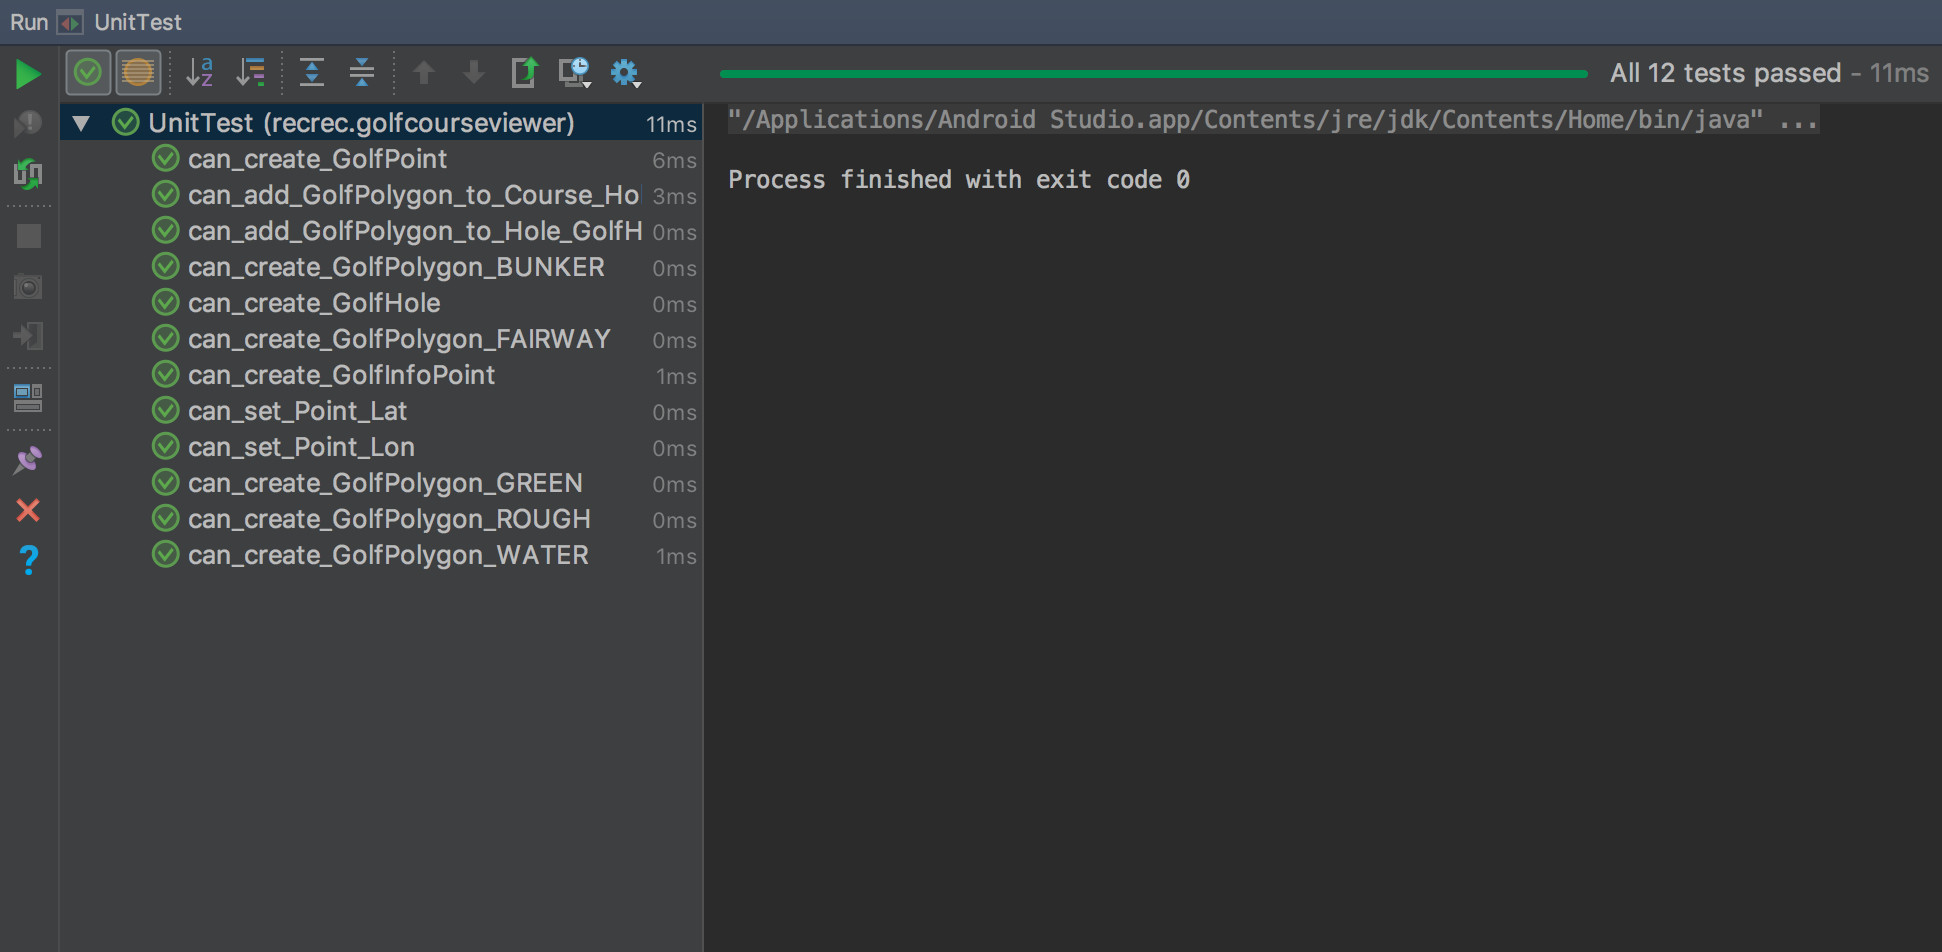
\includegraphics[scale=0.4]{AppUnitTest}
        \caption{JUnit tests being executed}
        \label{fig:junit}
    \end{figure}

    \newpage

    %===========================================================================

    \section{Zoning API Testing}
    \label{sec:mapper-api}

    This section describes the testing policies adopted in the
    \texttt{mapper-api} repository. The tools used for testing are described in
    Section \ref{sec:api-tools}. The layout of the test cases and history of
    the tests are shown respectively in Sections \ref{sec:api-cases} and
    \ref{sec:api-hist}.

    \subsection{Tools}
    \label{sec:api-tools}

    \textit{Moq} is used to validate input to function calls and produce
    expected output for functions that are not currently being tested. This
    allows you to focus on only a specific API function at a time, without
    worrying about it failing due to problems in other functions.
    
    \textit{xUnit} is then used to execute both unit and integration tests by
    making use of Moq to single out a specific API endpoint (and mocking the
    ouput of the others) and then asserting that the output of the tested
    function is as expected. The combination of these two tools allows powerful
    testing.

    The tests are automatically run by the Microsft Azure DevOps pipeline,
    described in Section \ref{sec:pipe}.

    \subsection{Test Cases}
    \label{sec:api-cases}

    The tests are located in the \texttt{/Test/TestSuite/API} folder. Every
    controller (and therefore, every use case) is tested in a separate
    \texttt{.cs} file, and the unit tests and integration tests are also
    separated into different files. As an example, the User controller has test
    cases in the \texttt{UserControllerUnitTests.cs} and
    \texttt{UserControllerIntegrationTests.cs} files.

    \subsection{History}
    \label{sec:api-hist}

    Figure \ref{fig:integration} shows the continuous integration being
    performed on Microsft Azure DevOps. You can see the deployment pipeline of
    building, testing and publishing the API.

    \begin{figure}[H]
        \centering
        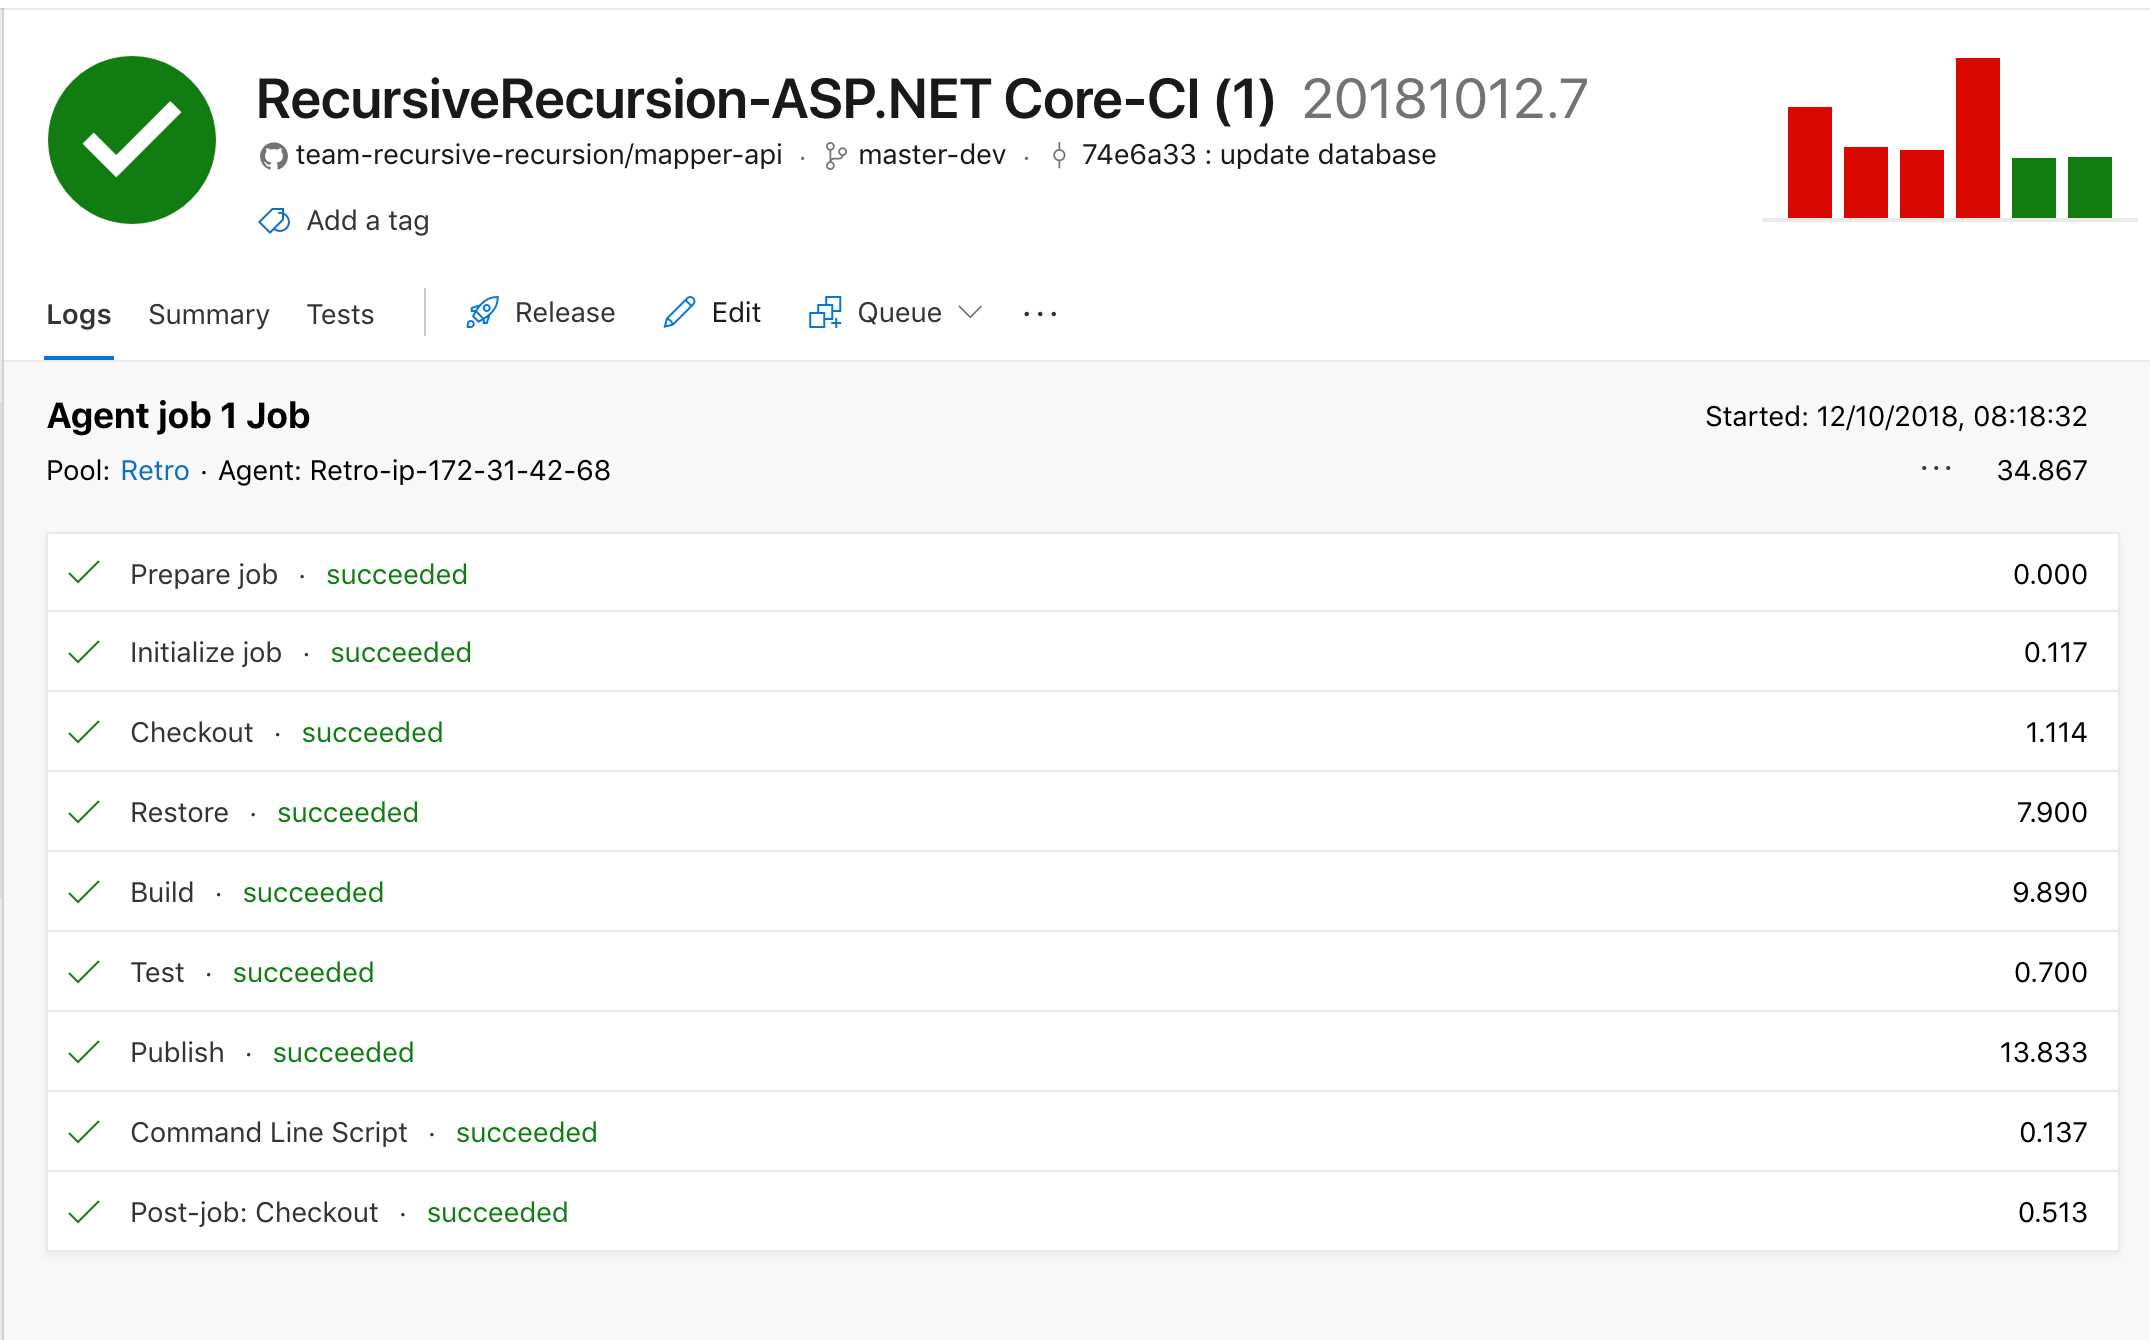
\includegraphics[scale=0.35]{Integration}
        \caption{Continuous integration}
        \label{fig:integration}
    \end{figure}

    \newpage

    %===========================================================================
    
    \section{References}

    \begin{enumerate}
        \item Microsoft Azure DevOps (\url{https://devops.azure.com})
        \item Software Requirements Specification
        (\url{https://github.com/team-recursive-recursion/documentation/raw/master/publish/requirements.pdf})
        \item Usability Report
        (\url{https://github.com/team-recursive-recursion/documentation/raw/master/publish/usabilitytest.pdf})
    \end{enumerate}


\end{document}
